\begin{enumerate}[label=\thesection.\arabic*,ref=\thesection.\theenumi]

\item Find the points on the curve $x^2+y^2-2x-3=0$ at which the tangents are parallel to the x-axis.
\label{chapters/12/6/3/19}
\\
\solution
Given that 
\begin{align}
	\vec{u} = \myvec{-1\\0},\,
	f = -3
\end{align}
Hence, the centre and radius are given as
\begin{align}
	\vec{c} = -\vec{u} = \myvec{1\\0},\,
	r = \sqrt{\norm{\vec{u}}^2 - f}
	  = 2
\end{align}
From \eqref{eq:conic_tangent_qk-circ},
the points of contact for the tangent are given by
\begin{align}
	\label{eq:chapters/12/6/3/19/eq3}
	\vec{q}_{ij} = \brak{\pm r\frac{\vec{n}_j}{\norm{\vec{n}_j}}-\vec{u}} \text{ i,j} = 1,2
\end{align}
Since, tangents are parallel to the x-axis, the normal is given as
\begin{align}
	\vec{n} = \myvec{0\\1}
\end{align}
Substituting in \eqref{eq:chapters/12/6/3/19/eq3} we get
\begin{align}
	\vec{q}_{11} &= \brak{\pm 2\myvec{0\\1} - \myvec{-1\\0}}\\
	&= \myvec{1\\-2},\myvec{1\\2}
\end{align}
Hence, the two points of contact are
\begin{align}
	\myvec{1\\2} \text{ and } \myvec{1\\-2}
\end{align}
See \figref{fig:chapters/12/6/3/19/Fig1}.
\begin{figure}[H]
	\begin{center} 
	    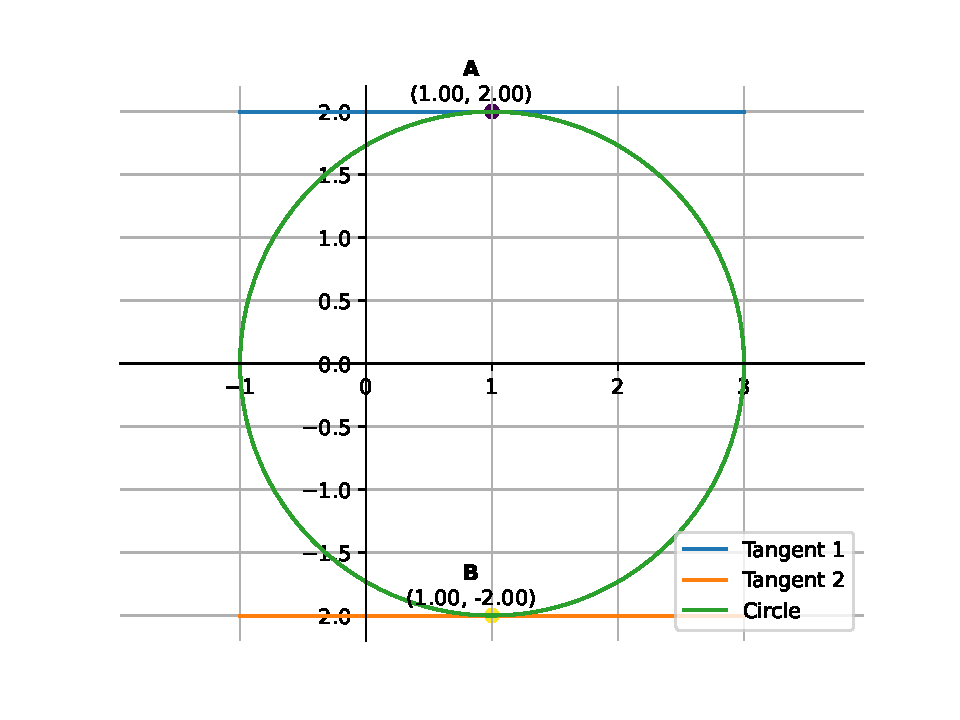
\includegraphics[width=0.75\columnwidth]{chapters/12/6/3/19/figs/fig.pdf}
	\end{center}
\caption{}
\label{fig:chapters/12/6/3/19/Fig1}
\end{figure}






















\item Find the equation of a circle of radius 5 which is touching another circle $x^2+y^2-2x-4y-20=0$ at (5,5).
\item The equation of the circle having centre at (3,-4) and touching the line $5x+12y-12=0$ is \makebox[1cm]{\hrulefill}                     
 \item Find the equation of the circle which touches both the axes in first quadrant and whose radius is $a$.
 \item Find the equation of the circle which touches x-axis and whose centre is $(1,2)$
 \item lf the lines $3x-4y+4=0$ and $6x-8y-7=0$ are tangents to a circle, then find the radius of the circle.
 \item Find the equation of a circle which touches  both the axes and the line $3x-4y+8=0$ and lies in the third quadrant.
\item At what points on the curve $x^2+y^2-2x-4y+1=0$, the tangents are parallel to the y-axis?
\item The shortest distance from the point (2,7) to the circle $x^2+y^2- 14x-10y-151=0$ is equal to 5.
\item lf the line $lx+my=1$ is a tangent to the circle $x^2+y^2=a^2$, then the point $(1,m)$ lies an a circle.

\end{enumerate}
